\documentclass{article}
\usepackage{tikz, comment}
\usepackage{pifont}
\usepackage{fontspec, pgfplots}
\usetikzlibrary{arrows, decorations.markings, decorations.pathreplacing}
\begin{comment}
:Title: Not defined yet
:Tags: area using parametric equations,parametric integral formula;cosine, cos ;polar form of a complex number;area using polar coordinates, polar integral formula ;moment
:Prob: 0.505;0.4831;0.4799;0.4789;0.4733
:Author: Prof.Hu Ji-shan, HKUST
:Slug: No name yet

Description Here.........
\end{comment}
\begin{document}\centering 

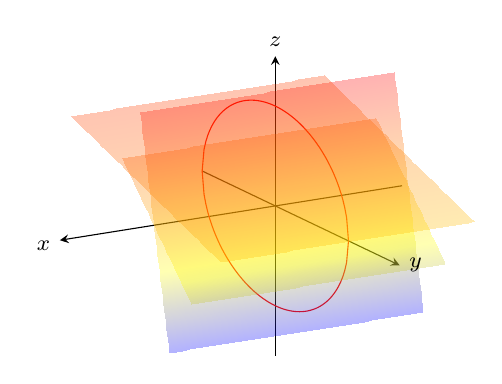
\begin{tikzpicture}[font=\footnotesize]
\pgfplotsset{compat=1.8}
\begin{axis}
[axis lines = center, view={150}{20}, ticks=none, scale=1,
axis background, xlabel = {$x$}, ylabel ={$y$}, zlabel ={$z$}, domain =-2:2, y domain =-2:2,
xmin =-1,
xmax =1.7,
ymin =-1,
ymax =1.7,
zmin =-1.5, 
zmax =1.5,
samples =10, samples y =40, z buffer = auto, 
every axis x label/.style={
    at={(ticklabel* cs:1)},
    anchor= east, yshift =-2
},
every axis y label/.style={
    at={(ticklabel* cs:1)},
    anchor= west,
},
every axis z label/.style={
    at={(ticklabel* cs:1)},
    anchor= south
}]

\addplot3 [data cs=cart, red, domain=0:1, y domain = 0:1] ({0},{y},{(1-y^2)^(1/2)});
\addplot3 [data cs=cart, red, domain=0:1, y domain = 0:1] ({0},{y},{-(1-y^2)^(1/2)});
\addplot3 [data cs=cart, red, domain=0:1, y domain = -1:0] ({0},{y},{(1-y^2)^(1/2)});
\addplot3 [data cs=cart, red, domain=0:1, y domain = -1:0] ({0},{y},{-(1-y^2)^(1/2)});

\addplot3[surf, opacity=0.3, shader=interp, samples=40, domain=-0.5:1.5, y domain = 0.75:1.15, z buffer=sort] ({x},{y},{(1-y*0.984808)/0.173648});%the plane, theta = 10^\circ

\addplot3[surf, opacity=0.3, shader=interp, samples=40, domain=-0.5:1.5, y domain = 0.5:1.45, z buffer=sort] ({x},{y},{(1-y*0.766044)/0.642788});%the plane, theta=40^\circ	

\addplot3[surf, opacity=0.3, shader=interp, samples=40, domain=-0.5:1.5, y domain = -0.2:1.85, z buffer=sort] ({x},{y},{(1-y*0.34202)/0.939693});%the plane, theta=70^\circ

\end{axis}

\end{tikzpicture}
\end{document}